\documentclass[11pt,a4paper]{article}
\usepackage[margin=26mm,headheight=15pt]{geometry}
\usepackage[T1]{fontenc}
\usepackage{amsmath,amsthm,mathtools}
\usepackage{newtxtext,newtxmath}
\usepackage{microtype,booktabs,array,longtable,enumitem}
\usepackage{xcolor,graphicx,fancyhdr}
\usepackage[most]{tcolorbox}
\usepackage{xurl}
\usepackage{float,needspace}
\usepackage[colorlinks=true,linkcolor=blue!45!black,citecolor=blue!45!black,urlcolor=blue!45!black]{hyperref}
\usepackage[nameinlink,noabbrev]{cleveref}
\numberwithin{equation}{section}
\newtheorem{theorem}{Theorem}[section]
\newtheorem{proposition}[theorem]{Proposition}
\newtheorem{corollary}[theorem]{Corollary}
\newtheorem{lemma}[theorem]{Lemma}
\theoremstyle{definition}
\newtheorem{definition}[theorem]{Definition}
\newtheorem{problem}{Research question}
\theoremstyle{remark}
\newtheorem{remark}[theorem]{Remark}
\newcommand{\C}{\mathbb C}
\newcommand{\R}{\mathbb R}
\newcommand{\N}{\mathbb N}
\newcommand{\e}{\mathrm e}
\newcommand{\ii}{\mathrm i}
\newcommand{\dd}{\,\mathrm d}
\newcommand{\B}{\mathcal B}
\newcommand{\Li}{\mathcal L}
\newcommand{\res}{\operatorname*{Res}}
\newcommand{\D}{\mathrm D}
\newcommand{\bn}{\boldsymbol n}
\newcommand{\bs}{\boldsymbol\sigma}
\newcommand{\bA}{\boldsymbol A}
\newcommand{\cF}{F_{\mathrm c}}
\newcommand{\cG}{G_{\mathrm c}}
\newcommand{\cU}{U_{\mathrm c}}
\newcommand{\norm}[1]{\left\lVert #1\right\rVert}
\newcommand{\abs}[1]{\left|#1\right|}
\newcommand{\set}[1]{\left\{#1\right\}}
\DeclareMathOperator{\Ei}{Ei}
\DeclareMathOperator{\Rea}{Re}
\DeclareMathOperator{\Ima}{Im}
\setlist{itemsep=3pt,topsep=5pt}
\setlength{\parskip}{4pt}
\setlength{\parindent}{15pt}
\setlength{\emergencystretch}{2em}
\pagestyle{fancy}
\fancyhf{}
\fancyhead[L]{\small Nonlinear Stokes transport}
\fancyhead[R]{\small Logarithmic inversion}
\fancyfoot[C]{\thepage}
\hypersetup{pdftitle={Nonlinear Stokes Transport under Logarithmic Inversion},pdfauthor={Research report prepared for Vladimir Reshetnikov},pdfsubject={Transseries, resurgence, analytic inversion, Stokes jumps, Lambert fold}}

\begin{document}
\hypersetup{pageanchor=false}
\begin{titlepage}
\thispagestyle{empty}
\vspace*{12mm}
{\sffamily\small RESEARCH REPORT\hfill 29 SEPTEMBER 2026\par}
\vspace{19mm}
{\Huge\bfseries Nonlinear Stokes Transport\par}
\vspace{4mm}
{\LARGE\bfseries under Logarithmic Inversion\par}
\vspace{9mm}
{\Large Convergent sector expansions, exact-core resurgence,\par
real reconstruction, and curvature-shifted fold scaling\par}
\vspace{13mm}
{\large Prepared for Vladimir Reshetnikov\par}
{\normalsize A companion research article for the ProveIt transseries program\par}
\vspace{14mm}
\begin{tcolorbox}[colback=blue!3,colframe=blue!35!black,boxrule=.5pt,arc=1mm]
\textbf{Principal result.} An additive exponentially small change of an analytic forward map induces a normally convergent, explicitly computable expansion of its inverse. A single contour argument supplies every mixed sector and a quantitative tail bound. In an Euler--logarithm family, an exact logarithmic core reduces the inverse correction to ordinary resurgent power series. Its finite Stokes transition, nonlinear real-averaging defect, and large-amplitude fold can then be analyzed in one framework.
\end{tcolorbox}
\vfill
\noindent\textbf{Status and scope.} The proofs are conventional mathematical proofs, not Lean-checked proofs. General resurgence closure, Lagrange inversion, and the Lambert branch point are established results and are credited as such. The explicitly formulated model problems below are resolved; priority or a community-wide ``breakthrough'' is not asserted. The proposed contributions are the quantitative synthesis and the model-specific consequences, whose independent novelty remains to be assessed.
\end{titlepage}
\hypersetup{pageanchor=true}

\begin{abstract}
Let $F$ be an analytic map with a chosen local inverse $G$, and perturb it by a finite sum $\sum_j\sigma_j\phi_j$. We prove a quantitative inverse-transport theorem: the perturbed inverse has coefficients
\[
 [\bs^{\bn}]G_{\bs}(x)=\frac{(-1)^N}{\bn!}
 \partial_x^{N-1}\!\left(G'(x)\prod_j\phi_j(G(x))^{n_j}\right),
 \qquad N=|\bn|\geq1,
\]
and, under an explicit boundary-separation hypothesis, the absolute tail above total degree $M$ is at most $\rho\chi^{M+1}/((M+1)(1-\chi))$. Specializing to exponential actions yields resonance-stable mixed sectors and commuting scalar transport flows. We then study
\[
 F_\pm(z)=z+a\log z+\sum_j b_j
 \int_{\Gamma_\pm}\frac{\e^{-zt}}{A_j-t}\dd t,
 \qquad A_j>0.
\]
Its forward jump is exactly $2\pi\ii\sum_jb_j\e^{-A_jz}$. In the coordinate $y+a\log y=x$, the inverse correction is an ordinary Gevrey--1 resurgent series; this is proved by verifying the hypotheses of established resurgent and summable implicit-function theorems with an explicit Borel kernel. The finite inverse jump is thereby completely determined, including all mixed sectors and their analytic realization. A sign-definite, order-$\e^{-2x}x^{2a}$ defect separates the arithmetic average of lateral inverses from the inverse of the arithmetic average. Finally, the normalized amplitude has convergence radius $\e^{-1}+O(g^{-2})$, a computable curvature-shifted fold, and the double-scaling limit $g(s+1)\to\sqrt{2\zeta+a/A}$. Exact symbolic checks, 100-digit numerical experiments, implementation formulas, and a research agenda accompany the proofs.
\end{abstract}
\tableofcontents
\newpage

\section{The problem, the repository, and the limits of the claims}
\label{sec:context}

\subsection{A concrete question beyond formal inversion}
A polynomial--logarithmic asymptotic expansion does not, by itself, record exponentially small choices of analytic realization. When two lateral sums of a divergent expansion differ, one must distinguish the forward jump from the jump of an inverse. Even an additive forward jump generally produces infinitely many nonlinear inverse sectors. The questions addressed here are precise:

\begin{enumerate}[label=(\roman*)]
\item Given the forward jump and one inverse branch, can every inverse sector be computed with an actual convergence theorem and a usable remainder?
\item Can logarithmic inversion be placed in ordinary Borel--Laplace theory without silently treating $\log x$ as a constant formal parameter?
\item Does arithmetic averaging of lateral branches commute with inversion, and what is the first error when it does not?
\item At what amplitude does the convergent sector expansion cease to be locally invertible, and which part of the forward asymptotics controls that transition?
\end{enumerate}

These questions are answered below for stated analytic hypotheses, and particularly for a finite-action Euler--logarithm model. They are not presented as previously named open conjectures in the general theory of transseries.

\subsection{Repository connection and provenance}
The inspected ProveIt snapshot is commit
\begin{center}
\texttt{04e06e032dff1966513bfba316966d52db3646b4}.
\end{center}
The transseries inventory identifies the consolidated volume in
\begin{quote}\small\ttfamily
Analysis/FabiusFunction/docs/\\
semi-formalized-research-frontiers/drafts/\\
series-and-transseries/Transseries\_And\_Inversion/
\end{quote}
and explicitly separates editorial consolidation from complete formalization \cite{repo}. Its stated topics include polynomial--logarithmic calculus, inversion around exact cores, Bell coefficients, analytic asymptotics, special-function inversion, and residual-to-error certificates. Named Lean modules include \texttt{LinLogCoreInversion.lean}, \texttt{RemainderTransport.lean}, \texttt{TransseriesFlat.lean}, and \texttt{UnitSeriesBellCoefficients.lean}.

The present work connects exact-core inversion to analytic Stokes transport. It does not reprove the repository's scale-uniqueness or Bell-normalization results as new results. The repository comparison is an inventory-level and statement-boundary comparison, not a claim of a line-by-line audit of the entire consolidated manuscript. In particular, absence of a theorem from the inventory is not evidence that it occurs nowhere in the repository.

\subsection{What is established background and what is contributed here}
Lagrange--B\"urmann inversion, analytic implicit functions, and the Euler Borel singularity are classical. Stability of resurgent and $1$-summable series under nonlinear operations, including implicit functions and functional inversion, is established in Sauzin's work \cite{sauzin2015,sauzin2014}. General transseries composition and inversion belong to a much broader theory \cite{edgar}. The Lambert function and its square-root branch point are also established \cite{dlmf}.

The research contribution proposed here is narrower: an explicit boundary-norm transport certificate, its resonance-stable multi-action form, an exact Borel kernel for logarithmic-core normalization, a quantitative nonlinear averaging defect, an action-recovery procedure that remains valid at nonlinear resonances, and a curvature-sensitive amplitude-fold analysis. Each statement has explicit hypotheses and a proof. Several are refinements or applications of classical machinery rather than new general foundations. Their priority has not been established by an exhaustive literature review.

\begin{remark}[Two different meanings of convergence]
There will be a \emph{convergent Taylor series in exponential amplitudes} whose coefficients are analytic functions. The asymptotic expansions of those coefficient functions in inverse powers may diverge. Normal convergence of the sector sum does not imply ordinary convergence of the entire doubly expanded transseries.
\end{remark}

\section{A quantitative analytic inverse-transport theorem}
\label{sec:transport}

\subsection{Boundary separation}
Write $D(g,\rho)=\{z:|z-g|<\rho\}$. Let $F$ and $\phi_1,\ldots,\phi_d$ be holomorphic on a neighborhood of its closure. Fix $x=F(g)$ and suppose that $F(z)-x$ has exactly one zero in the disk, counted with multiplicity. Thus its zero at $g$ is simple. Set
\begin{align}
 m&=\min_{|z-g|=\rho}|F(z)-x|>0,\label{eq:m}\\
 M_j&=\max_{|z-g|=\rho}|\phi_j(z)|,\qquad
 \chi=\frac{\sum_{j=1}^d|\sigma_j|M_j}{m}.
 \label{eq:chi}
\end{align}
The same maximum bounds hold throughout the disk.

\begin{theorem}[Certified finite perturbation of an inverse]
\label{thm:transport}
If $\chi<1$, the equation
\begin{equation}
 F(z)+\sum_{j=1}^d\sigma_j\phi_j(z)=x
 \label{eq:perturbed}
\end{equation}
has exactly one solution in $D(g,\rho)$, counted with multiplicity. The solution $G_{\bs}(x)$ is holomorphic in the amplitudes on the open weighted ball defined by $\chi<1$. For $G=G_{\boldsymbol0}$, let $\bn=(n_1,\ldots,n_d)$, $N=|\bn|$, and $\bn!=\prod_jn_j!$. Then
\begin{equation}
 G_{\bs}(x)=G(x)+\sum_{\bn\neq\boldsymbol0}\bs^{\bn}C_{\bn}(x),
 \qquad
 C_{\bn}(x)=\frac{(-1)^N}{\bn!}
 \partial_x^{N-1}\left[G'(x)\prod_j\phi_j(G(x))^{n_j}\right].
 \label{eq:transport}
\end{equation}
The series is absolutely convergent. More precisely,
\begin{equation}
 \sum_{|\bn|=N}|\bs^{\bn}C_{\bn}(x)|
 \leq\frac{\rho}{N}\chi^N\quad(N\geq1),
 \label{eq:homogeneous-bound}
\end{equation}
and truncation at total degree $M\geq0$ has absolute error at most
\begin{equation}
 \rho\sum_{N=M+1}^{\infty}\frac{\chi^N}{N}
 \leq \frac{\rho\chi^{M+1}}{(M+1)(1-\chi)}.
 \label{eq:tail}
\end{equation}
Here derivatives in \eqref{eq:transport} refer to the local inverse germ near the fixed $x$. All conclusions are locally uniform when the data and a strict bound $\chi<1$ are uniform.
\end{theorem}

\begin{proof}
Put $H(z)=F(z)-x$ and $E(z)=\sum_j\sigma_j\phi_j(z)$. On the boundary $|E|<|H|$, so Rouch\'e's theorem gives exactly one zero of $H+E$ inside, counted with multiplicity. It must be simple. The analytic implicit-function theorem supplies local holomorphic dependence on the parameters; uniqueness glues these local solutions throughout the weighted ball.

The residue formula for the unique zero gives
\[
 G_{\bs}(x)-G(x)=\frac1{2\pi\ii}\int_{|z-g|=\rho}
 z\left(\frac{H'(z)+E'(z)}{H(z)+E(z)}-\frac{H'(z)}{H(z)}\right)\dd z.
\]
On a thin annulus containing the contour, the uniformly convergent power series for $\log(1+E/H)$ defines a single-valued logarithm. Integration by parts around the closed contour yields
\begin{align}
 G_{\bs}(x)-G(x)
 &=-\frac1{2\pi\ii}\int_{|z-g|=\rho}\log\left(1+\frac{E(z)}{H(z)}\right)\dd z\notag\\
 &=\sum_{N\geq1}\frac{(-1)^N}{2\pi\ii N}
 \int_{|z-g|=\rho}\frac{E(z)^N}{(F(z)-x)^N}\dd z.
 \label{eq:contour-transport}
\end{align}
The only pole of an individual integrand inside the contour is at $g$. On a sufficiently small circle around $g$, make the local change of coordinate $w=F(z)$, $z=G(w)$. Cauchy's differentiation formula gives
\[
 \frac1{2\pi\ii}\int\frac{E(z)^N}{(F(z)-x)^N}\dd z
 =\frac1{(N-1)!}\partial_x^{N-1}\left[G'(x)E(G(x))^N\right].
\]
The multinomial expansion of $E^N$ proves \eqref{eq:transport}.

For absolute convergence, do not estimate a differentiated expression. Estimate its contour representation instead. After taking the sum of the absolute values of the degree-$N$ monomials, the multinomial theorem bounds the numerator by $(\sum_j|\sigma_j|M_j)^N$. The contour has length $2\pi\rho$ and its denominator has modulus at least $m^N$. This proves \eqref{eq:homogeneous-bound}. Summation proves \eqref{eq:tail}. The same estimates justify every interchange and give local uniformity.
\end{proof}

\subsection{An easily evaluated sufficient certificate}
\begin{corollary}[Derivative-disk certificate]
\label{cor:disk}
Suppose $c=F'(g)\neq0$ and
\begin{equation}
 \sup_{|z-g|\leq\rho}|F'(z)-c|\leq\vartheta|c|,
 \qquad 0\leq\vartheta<1.
 \label{eq:derivative-disk}
\end{equation}
Then the hypotheses preceding \cref{thm:transport} hold and one may replace $m$ by the lower bound $|c|(1-\vartheta)\rho$. For exponential perturbations $\phi_j(z)=\e^{-A_jz}$ one may use
\begin{equation}
 M_j\leq |\e^{-A_jg}|\e^{|A_j|\rho}.
 \label{eq:exp-norm}
\end{equation}
\end{corollary}
\begin{proof}
Integrating $F'-c$ on the segment joining two points of the convex disk shows
\[
 |F(z_1)-F(z_2)|\geq |c|(1-\vartheta)|z_1-z_2|.
\]
Thus $F$ is injective there, the zero at $g$ is simple, and the asserted boundary lower bound follows by taking $z_2=g$. The exponential bound is immediate.
\end{proof}

\begin{remark}[A certificate, not merely a formal identity]
The coefficient formula is a form of classical Lagrange inversion. The usable conclusion here is the package: a specified inverse branch, an admissible amplitude domain, absolute mixed-sector convergence, and the explicit factor $1/(M+1)$ in the tail. None of these is inferred solely from formal substitution.
\end{remark}

\subsection{Countably many analytic perturbations}
\begin{corollary}[Weighted summable families]
\label{cor:countable}
The theorem remains valid for a countable family when
$\sum_j|\sigma_j|M_j<m$. The inverse depends holomorphically on the corresponding weighted $\ell^1$ parameter, after zero-norm coordinates are omitted. Its expansion over finite-support multi-indices converges absolutely and obeys \eqref{eq:homogeneous-bound}--\eqref{eq:tail}.
\end{corollary}
\begin{proof}
The perturbation series converges normally on the disk by the Weierstrass test. The strict contour inequality persists. Finite partial sums satisfy all estimates uniformly, and their roots converge to the unique root of the full equation. For each degree, the absolute multinomial majorant passes to the limit by monotone convergence. The contour logarithm is a normally convergent series of continuous homogeneous polynomials on the weighted Banach space, which proves holomorphy.
\end{proof}
This analytic extension does not automatically prove a countable-action resurgence theorem. That requires additional Borel-plane hypotheses.

\section{Exponential actions, resonances, and commuting flows}
\label{sec:actions}

\subsection{Every mixed sector in one formula}
Let $\phi_j(z)=\e^{-A_jz}$ and define $S_{\bn}=\sum_jn_jA_j$. Then \cref{thm:transport} becomes
\begin{equation}
 C_{\bn}(x)=\frac{(-1)^N}{\bn!}
 \partial_x^{N-1}\left[G'(x)\e^{-S_{\bn}G(x)}\right].
 \label{eq:actions}
\end{equation}
When $S_{\bn}\neq0$, an equivalent form is
\begin{equation}
 C_{\bn}(x)=\frac{(-1)^{N+1}}{S_{\bn}\bn!}
 \partial_x^N\e^{-S_{\bn}G(x)}.
 \label{eq:bell-form}
\end{equation}
The first form remains valid even when complex actions cancel to $S_{\bn}=0$. In particular, there is no denominator of the form $n_1A_1-n_2A_2$.

For one action $A$, write $g=G(x)$ and $g_k=G^{(k)}(x)$. The first four coefficients, with the amplitude omitted, are
\begin{align}
 C_1&=-\e^{-Ag}g_1,\notag\\
 C_2&=\tfrac12\e^{-2Ag}(g_2-2Ag_1^2),\notag\\
 C_3&=-\tfrac16\e^{-3Ag}(g_3-9Ag_1g_2+9A^2g_1^3),\label{eq:first-sectors}\\
 C_4&=\tfrac1{24}\e^{-4Ag}
 \left(g_4-16Ag_1g_3-12Ag_2^2
       +96A^2g_1^2g_2-64A^3g_1^4\right).\notag
\end{align}
These are identities between analytic functions, not only asymptotic expressions.

\begin{proposition}[Collision stability]
\label{prop:collision}
For finitely many actions in a compact set, the coefficients and the analytic sum vary holomorphically with the actions whenever the strict boundary certificate is uniform. If two actions coalesce, their two amplitudes combine by ordinary addition. If distinct multi-indices have the same total action, their contributions are added without a singular limit.
\end{proposition}
\begin{proof}
The functions $\e^{-A_jz}$ depend holomorphically on $A_j$, and their boundary norms are uniformly bounded on compact action sets. Apply the contour formula and its majorant. At $A_1=A_2=A$, the forward perturbation is exactly $(\sigma_1+\sigma_2)\e^{-Az}$. Uniqueness identifies its inverse with the limit of the two-action inverse. Equal total actions in \eqref{eq:actions} simply give terms with the same exponential factor.
\end{proof}

For example, with actions $A$ and $2A$, action $2A$ receives both the primitive contribution
$-\sigma_2\e^{-2Ag}g_1$ and the induced contribution
$\frac12\sigma_1^2\e^{-2Ag}(g_2-2Ag_1^2)$.
Action $3A$ receives the $\sigma_1\sigma_2$ term
\[
 \sigma_1\sigma_2\e^{-3Ag}(g_2-3Ag_1^2)
\]
and the $\sigma_1^3$ term from \eqref{eq:first-sectors}. Resonance changes bookkeeping; it does not create a new free amplitude.

\subsection{The scalar transport hierarchy}
\begin{proposition}[Commuting inverse-deformation flows]
\label{prop:flows}
On every certified branch,
\begin{equation}
 \partial_{\sigma_j}G_{\bs}
 =-\phi_j(G_{\bs})\partial_xG_{\bs}.
 \label{eq:flow}
\end{equation}
These are commuting evolutionary flows. Locally, if
$\mathcal T_E(G)=(G^{-1}+E)^{-1}$ with coherent choices of inverse branch, then
\begin{equation}
 \mathcal T_E\mathcal T_D(G)=\mathcal T_{E+D}(G)
 =\mathcal T_D\mathcal T_E(G).
 \label{eq:group}
\end{equation}
\end{proposition}
\begin{proof}
Differentiate the defining equation with respect to $x$ and $\sigma_j$. Its nonzero $z$-derivative is the same denominator in both formulas, proving \eqref{eq:flow}. For a direct commutator check, let
$V_j[G]=-\phi_j(G)G_x$. Its linearization is
\[
 \D V_j[G](H)=-\phi_j'(G)HG_x-\phi_j(G)H_x.
\]
Substitution of $H=V_k[G]$ gives
\[
 \D V_j[G](V_k[G])=
 (\phi_j'\phi_k+\phi_j\phi_k')(G)G_x^2
 +\phi_j(G)\phi_k(G)G_{xx},
\]
which is symmetric in $j,k$. Equation \eqref{eq:group} also follows immediately by taking the forward inverse before adding the perturbations.
\end{proof}

For exponential $\phi_j$, \eqref{eq:flow} is a scalar quasilinear transport hierarchy. The factor $G_x$ is essential: the ordinary one-dimensional vector fields $-\e^{-A_jg}\partial_g$ are different objects and need not commute. Nor does this local additive model imply that arbitrary Stokes operators in differential systems commute.

\subsection{Leading sectors on a logarithmic scale}
\begin{proposition}[Action transport and tree coefficients]
\label{prop:leading}
Suppose on a sector containing the positive real axis that
\begin{equation}
 G(x)=x-a\log x+O(x^{-1}\log x),
 \label{eq:Gleading}
\end{equation}
with differentiated asymptotic estimates. For fixed positive actions and a fixed nonzero multi-index,
\begin{equation}
 C_{\bn}(x)=
 -\frac{S_{\bn}^{N-1}}{\bn!}\,
 \e^{-S_{\bn}x}x^{aS_{\bn}}
 \left(1+O\left(\frac{\log x}{x}\right)\right)
 \quad(x\to+\infty).
 \label{eq:leading-sector}
\end{equation}
Thus inversion preserves each additive exponential action and changes its algebraic prefactor by $x^{aS_{\bn}}$.
\end{proposition}
\begin{proof}
The assumptions give $G'=1+O(x^{-1})$ and $G^{(k)}=O(x^{-k})$ for $k\geq2$, with harmless logarithmic factors at subsequent orders. In $\partial_x^{N-1}(G'\e^{-SG})$, the leading term is
$(-S)^{N-1}(G')^N\e^{-SG}$; all other terms contain higher derivatives of $G$ and are lower order. Finally,
$\e^{-SG}=\e^{-Sx}x^{aS}(1+O(x^{-1}\log x))$. The sign in \eqref{eq:actions} is
$(-1)^N(-1)^{N-1}=-1$.
\end{proof}

For $F(z)=z$, formula \eqref{eq:leading-sector} is exact, without its error factor. For one action its coefficients are
$-(nA)^{n-1}/n!$, the familiar rooted-tree coefficients of Lambert inversion. This combinatorial appearance is classical; its use here makes the leading mixed Stokes sectors transparent. For perturbations $z^{\beta_j}\e^{-A_jz}$ on a fixed logarithm branch, the identical proof replaces the power $x^{aS}$ by $x^{aS+\sum_jn_j\beta_j}$.

\section{An analytic Euler--logarithm family}
\label{sec:euler}

\subsection{Conventions for lateral Borel sums}
Our formal Borel transform is
\begin{equation}
 \B\left(\sum_{n\geq0}c_nz^{-n-1}\right)(t)
 =\sum_{n\geq0}\frac{c_n}{n!}t^n.
 \label{eq:borel}
\end{equation}
For $A>0$, define the formal Euler series and its nonsingular directional sums by
\begin{equation}
 \widehat U_A(z)=\sum_{n\geq0}\frac{n!}{A^{n+1}z^{n+1}},
 \qquad
 U_{A,\theta}(z)=\int_0^{\e^{\ii\theta}\infty}
 \frac{\e^{-zt}}{A-t}\dd t,
 \label{eq:euler}
\end{equation}
where $\theta\not\equiv0\pmod{2\pi}$ and $\Rea(z\e^{\ii\theta})>0$. We use a small positive angle for $+$ and a small negative angle for $-$, analytically continued to their common domain around $z>0$. Equivalently, the upper contour passes \emph{above} the positive Borel pole while travelling from $0$ to $+\infty$.

\begin{lemma}[Euler jump, differential equation, and remainder]
\label{lem:euler}
With these conventions,
\begin{align}
 U_{A,+}(z)-U_{A,-}(z)&=2\pi\ii\e^{-Az},\label{eq:Ujump}\\
 U_{A,\theta}'(z)+A U_{A,\theta}(z)&=z^{-1}.\label{eq:Uode}
\end{align}
If $0<|\theta|<\pi/2$, $\mu=\Rea(z\e^{\ii\theta})>0$, and $N\geq0$, then
\begin{equation}
 \left|U_{A,\theta}(z)-\sum_{n=0}^{N-1}\frac{n!}{A^{n+1}z^{n+1}}\right|
 \leq \frac{N!}{A^{N+1}|\sin\theta|\mu^{N+1}}.
 \label{eq:euler-bound}
\end{equation}
On the positive real axis,
\begin{equation}
 U_{A,\pm}(z)=\e^{-Az}\big(\Ei(Az)\pm\pi\ii\big).
 \label{eq:Ei}
\end{equation}
\end{lemma}
\begin{proof}
The upper path followed by the reversed lower path winds clockwise around $A$. The residue of $(A-t)^{-1}\e^{-zt}$ is $-\e^{-Az}$, so its clockwise integral is $2\pi\ii\e^{-Az}$. Large arcs vanish in the common Laplace domain. Differentiation under the integral and $t/(A-t)=A/(A-t)-1$ give \eqref{eq:Uode}.

For the remainder, use the exact geometric identity
\[
 \frac1{A-t}=\sum_{n=0}^{N-1}\frac{t^n}{A^{n+1}}
 +\frac{t^N}{A^N(A-t)}.
\]
On the ray $t=r\e^{\ii\theta}$ one has $|A-t|\geq A|\sin\theta|$. Integration of the remainder is bounded by
$A^{-N-1}|\sin\theta|^{-1}\int_0^\infty r^N\e^{-\mu r}\dd r$, proving \eqref{eq:euler-bound}. The finite polynomial integrals are $n!z^{-n-1}$.
Finally $\e^{-Az}\Ei(Az)$ solves \eqref{eq:Uode}; the upper and lower indentation contributions are respectively $+\pi\ii\e^{-Az}$ and $-\pi\ii\e^{-Az}$, establishing \eqref{eq:Ei}.
\end{proof}

\subsection{The forward and inverse maps}
Fix $a,b_1,\ldots,b_d\in\C$ and $A_1,\ldots,A_d>0$. On a fixed logarithm branch set
\begin{equation}
 F_\pm(z)=z+a\log z+\sum_{j=1}^d b_jU_{A_j,\pm}(z).
 \label{eq:Fpm}
\end{equation}
Then the exact forward transition is
\begin{equation}
 F_+(z)=F_-(z)+2\pi\ii\sum_jb_j\e^{-A_jz}.
 \label{eq:Fjump}
\end{equation}
For real parameters define the real central forward map
\begin{equation}
 \cF(z)=z+a\log z+\sum_jb_j\e^{-A_jz}\Ei(A_jz),
 \qquad F_\pm=\cF\pm\pi\ii\sum_jb_j\e^{-A_jz}.
 \label{eq:central}
\end{equation}
The notation ``central'' denotes this explicitly specified arithmetic average. It is not a definition of general \'{E}calle median summation.

\begin{proposition}[Selected inverse branches at infinity]
\label{prop:existence}
On each sufficiently narrow closed subsector about the positive real axis, and for sufficiently large $|x|$, the maps in \eqref{eq:Fpm} have uniquely selected inverse branches near $x-a\log x$. They satisfy
\begin{equation}
 G_\pm(x)=x-a\log x+O(x^{-1}\log x),
 \qquad G_\pm'(x)=1+O(x^{-1}).
 \label{eq:inverse-exists}
\end{equation}
The same holds for $\cG=\cF^{-1}$ when it is defined by \eqref{eq:central}. All these branches have the same polynomial--logarithmic Poincar\'e expansion.
\end{proposition}
\begin{proof}
Choose upper and lower Laplace rays with angles small enough that both Laplace exponents have uniformly positive real part on a slightly larger $z$-sector. Equation \eqref{eq:euler-bound} gives $U_A=O(z^{-1})$, and the differentiated integrals give $U_A^{(k)}=O(z^{-k-1})$ for each fixed $k$. Hence $F'(z)=1+O(z^{-1})$.

At $z_0=x-a\log x$, the residual $F(z_0)-x$ is $O(x^{-1}\log x)$. On a disk about $z_0$ of radius $K|x|^{-1}(1+|\log x|)$, subtracting the affine map $z-z_0$ leaves this residual plus a term with derivative $O(x^{-1})$. With $K$ sufficiently large, Rouch\'e's theorem gives one root in the disk. The derivative remains nonzero, so these roots form a holomorphic branch. The inverse derivative formula proves the displayed derivative estimate.

Substitution of a finite power--logarithm ansatz is triangular: its next coefficient appears linearly with coefficient $1$. The Euler remainder estimate and the same disk argument transfer the finite residual to an inverse error. Exponentials in \eqref{eq:Fjump} are smaller than every algebraic order on the stated sectors, so the recursively determined expansions agree. Differentiated estimates follow from Cauchy's formula on slightly smaller sectors.
\end{proof}

\section{Exact-core normalization and ordinary resurgence}
\label{sec:core}

\subsection{Removing the logarithm before applying the Borel transform}
Define the exact core $H_a$ by the selected branch
\begin{equation}
 y=H_a(x),\qquad y+a\log y=x,
 \qquad y=x-a\log x+O(x^{-1}\log x).
 \label{eq:core}
\end{equation}
For real $a>0$ and large real $x$, this is
$y=aW_0(\e^{x/a}/a)$; for $a=0$ it is $y=x$. The implicit definition is preferable for general complex parameters because it records the branch selection.

Write the desired inverse as $G_\pm(x)=y+r_\pm(y)$. Its defining equation becomes
\begin{equation}
 r+a\log(1+r/y)+\sum_jb_jU_{A_j,\pm}(y+r)=0.
 \label{eq:core-implicit}
\end{equation}
There is no $\log y$ left in this equation. Its unique formal solution is an ordinary power series
$\widehat r(y)\in y^{-1}\C[[y^{-1}]]$.

\subsection{The Borel kernel and summability theorem}
For clarity, a formal series $\sum_{n\geq1}c_ny^{-n}$ is \emph{Gevrey--1} when $|c_n|\leq CK^n n!$ for some $C,K$. It is \emph{$1$-summable} in an angular interval when its convergent Borel germ continues in those directions with uniform exponential growth on smaller closed intervals, so its Laplace integral defines an analytic sum. It is \emph{$\Omega$-resurgent} when that germ admits continuation along every path starting at the origin and avoiding $\Omega$ thereafter, with branches recorded on the associated lifted surface. These are the conventions used in the cited implicit-function theorems \cite{sauzin2015,sauzin2014}.

Let
\begin{equation}
 \Omega=\left\{\sum_jn_jA_j:n_j\in\N\right\}.
 \label{eq:Omega}
\end{equation}
It includes $0$, is stable under addition, and is closed and locally finite: below any fixed positive bound every $n_j$ has a finite bound. This remains true when the ratios of the positive actions are irrational.

\begin{theorem}[Resurgent correction in the exact-core coordinate]
\label{thm:core}
The formal solution $\widehat r$ of \eqref{eq:core-implicit} is Gevrey--1 and $\Omega$-resurgent. In particular, its Borel transform continues along paths avoiding $\Omega$, in the usual lifted-path sense. It is $1$-summable in every closed angular interval avoiding the positive Borel ray. The upper and lower sums are exactly the corrections $r_\pm$ selected in \eqref{eq:core-implicit}, and therefore
\begin{equation}
 G_\pm(x)=H_a(x)+
 \big(\operatorname{Sum}_{\pm}\widehat r\big)(H_a(x)).
 \label{eq:core-sum}
\end{equation}
The key parameter-dependent Borel kernel, with $r$ treated as an independent analytic parameter, is
\begin{equation}
 K(t,r)=a\frac{1-\e^{-rt}}{t}
       +\sum_j\frac{b_j\e^{-rt}}{A_j-t}.
 \label{eq:kernel}
\end{equation}
The singularity at $t=0$ in the first term is removable. The assertion gives a set of \emph{possible} Borel singularities, not a claim that every point of $\Omega$ is singular.
\end{theorem}

\begin{proof}
Put $v=y^{-1}$. The formal left side of \eqref{eq:core-implicit} belongs to $\C[[v,r]]$, has zero constant term, and its $r$-derivative at $(v,r)=(0,0)$ is $1$. The formal implicit-function theorem gives a unique $r\in v\C[[v]]$.

For fixed $r$, direct termwise Borel transformation gives
\[
 \B_y\log(1+r/y)=\frac{1-\e^{-rt}}{t},\qquad
 \B_y\widehat U_A(y+r)=\frac{\e^{-rt}}{A-t}.
\]
For the second identity one can either expand $(y+r)^{-n-1}$ or use
$\widehat U_A(y+r)=\sum_{k\geq0}r^k\widehat U_A^{(k)}(y)/k!$ and
$\B_y\widehat U_A^{(k)}=(-t)^k/(A-t)$. This proves \eqref{eq:kernel}. It is the Borel transform of the part of the implicit equation other than its constant-in-$y$ term $r$.

We now verify, rather than assume, the analytic-parameter hypotheses of the established implicit theorems. On every compact subset of the lifted Borel surface avoiding $\Omega$, the projection $t$ is bounded and its distance from the finitely many $A_j$ is positive. For $k\geq1$, the coefficient of $r^k$ in $K$ is
\begin{equation}
 \frac{a(-1)^{k+1}t^{k-1}}{k!}
 +\sum_j\frac{b_j(-t)^k}{k!(A_j-t)}.
 \label{eq:kernel-coeff}
\end{equation}
Its compact seminorm is bounded geometrically in $k$ (in fact with an additional factorial denominator). The $k=0$ coefficient has the same continuation property. Thus the implicit expression is an analytic power series in $r$ with coefficients in the $\Omega$-resurgent algebra. Sauzin's resurgent implicit-function theorem, Theorem~4 of \cite{sauzin2015}, applies.

For summability, choose a closed interval of Borel angles not meeting the positive ray and a sufficiently small disk at the origin. On their union, each $(A_j-t)^{-1}$ is bounded; outside a bounded set it is $O(|t|^{-1})$. For any fixed $\tau>0$,
$|t|^k/k!\leq\tau^{-k}\e^{\tau|t|}$. Equation \eqref{eq:kernel-coeff} consequently has a uniform exponential-type bound $CB^k\e^{\tau|t|}$. This verifies the coefficient-norm hypothesis of the summable implicit-function theorem, Theorem~$4'$ in \cite{sauzin2015}. Its conclusion is a $1$-summable formal correction, and summation gives a solution of the analytically summed equation.

That summed equation is precisely \eqref{eq:core-implicit}, because the displayed kernel has Laplace sum
$a\log(1+r/y)+\sum_jb_jU_{A_j,\theta}(y+r)$ when $y$ is large and $r$ is bounded. The solution tends to $0$ at infinity and is the unique small solution by the ordinary analytic implicit-function theorem or the disk argument of \cref{prop:existence}. It must therefore be $r_\pm$. Gevrey--1 asymptotics is part of $1$-summability. This proves \eqref{eq:core-sum}.
\end{proof}

\begin{remark}[What was imported]
The deep continuation estimates behind the general resurgent implicit-function theorem are not new here. The contribution of \cref{thm:core} is the exact-core reduction and the explicit verification by \eqref{eq:kernel}. One must not replace this verification by an unsupported assertion that ordinary Borel summability automatically handles arbitrary power--logarithm substitutions.
\end{remark}

\subsection{Explicit perturbative coefficients}
For one Euler pole at $A=1$, write $b=b_1$. The beginning of the ordinary core correction is
\begin{align}
 \widehat r(y)={}&-\frac{b}{y}+\frac{b(a-1)}{y^2}
 -\frac{b(a^2-a+b+2)}{y^3}\notag\\
 &+\frac{b(2a^3-2a^2+5ab+4a-6b-12)}{2y^4}
 +O(y^{-5}).
 \label{eq:core-coefficients}
\end{align}
This is a formal $O$ notation, or an asymptotic one after lateral summation. The accompanying program computes six coefficients by exact symbolic recursion.

Returning to $x$ and writing $L=\log x$ gives
\begin{align}
 \widehat G(x)={}&x-aL+\frac{a^2L-b}{x}\notag\\
 &+\frac{\frac12a^3L^2-(a^3+ab)L+ab-b}{x^2}
 +O\!\left(\frac{(1+L)^3}{x^3}\right).
 \label{eq:polylog-coefficients}
\end{align}
For several actions, the coefficient $b$ of $x^{-1}$ in the forward Euler part is replaced by $B_1=\sum_jb_j/A_j$, and its coefficient of $x^{-2}$ by $B_2=\sum_jb_j/A_j^2$. The numerator at order $x^{-2}$ in the inverse becomes
$\frac12a^3L^2-(a^3+aB_1)L+aB_1-B_2$.

A direct recursion avoiding any branch of $W$ is also useful. Put $v=x^{-1}$ and
$G=x(1+w)$, with $w=-aLv+O(v^2)$. In the one-pole case the formal equation is
\begin{equation}
 w=-aLv-av\log(1+w)
 -b\sum_{n\geq0}n!\,v^{n+2}(1+w)^{-n-1}.
 \label{eq:polylog-recursion}
\end{equation}
At each power of $v$, the right-hand side uses only coefficients already known. This produces the polynomial--logarithm coefficients in \eqref{eq:polylog-coefficients}. It is an algorithm for formal coefficients, not a license to sum a divergent power series numerically without a summation or truncation rule.

\section{Exact inverse Stokes transitions and real reconstruction}
\label{sec:jump}

\subsection{A finite-jump theorem, not just a first-order estimate}
\begin{theorem}[Complete inverse transition for the Euler--logarithm model]
\label{thm:jump}
Let $G=G_-$ be the branch of \cref{prop:existence}, $\Delta_j=2\pi\ii b_j$, $N=|\bn|$, and $S_{\bn}=\sum_jn_jA_j$. For sufficiently large positive $x$,
\begin{equation}
 G_+(x)-G_-(x)=
 \sum_{\bn\neq0}\frac{(-1)^N\boldsymbol\Delta^{\bn}}{\bn!}
 \partial_x^{N-1}\left[G_-'(x)\e^{-S_{\bn}G_-(x)}\right].
 \label{eq:exact-Stokes}
\end{equation}
The sum is absolutely convergent and has the quantitative tail \eqref{eq:tail} for any valid disk certificate. All inverse sectors are determined by the $d$ forward constants $b_j$ and the chosen base branch. There are no additional independently selectable inverse-sector constants in this problem.
\end{theorem}
\begin{proof}
Equation \eqref{eq:Fjump} is exact. The derivatives of $F_-$ tend to those of the identity on every fixed-radius disk about its large inverse root. Thus \cref{cor:disk} holds with $\vartheta\to0$, while
$\sum_j|\Delta_j|M_j\to0$. Apply \cref{thm:transport}. Its root agrees with the selected $G_+$ by uniqueness. Its coefficients are \eqref{eq:actions}. The last assertion follows from uniqueness of this holomorphic amplitude family, not from a count of symbols in a formal ansatz.
\end{proof}

For one pole and action $1$,
\begin{equation}
 G_+(x)-G_-(x)
 =-2\pi\ii b\,\e^{-x}x^a
 \left[1+\frac{b-a-a^2\log x}{x}
 +O\!\left(\frac{(1+\log x)^2}{x^2}\right)\right]
 +O\!\left(\e^{-2x}x^{2\Rea a}\right).
 \label{eq:leading-jump}
\end{equation}
Here the bracket describes the perturbative expansion of the first sector; the final term bounds the remaining sectors on the real axis. When parameters are real, a better parity-resolved description is available by centering the expansion, as below.

\begin{remark}[Finite transition versus alien derivatives]
Equation \eqref{eq:exact-Stokes} computes the actual lateral transition. It does not, by itself, identify the local singular expansion at every individual Borel singularity or resolve every decomposition into alien derivatives. Those finer questions matter especially when different primitive actions or their multiples coincide.
\end{remark}

\subsection{Parity in a centrally based expansion}
Assume now that $a,b$ are real, there is one pole at action $1$, and $x$ is sufficiently large and real. Set
\[
 g=\cG(x),\qquad p=\pi\ii b,
 \qquad G_\sigma=(\cF+\sigma\e^{-z})^{-1}.
\]
The coefficients $C_n$ below are based on $\cG$, not on $G_-$. Thus
$G_+=G_p$ and $G_-=G_{-p}$. Every $C_n(x)$ is real.

\begin{theorem}[Nonlinear real-averaging defect]
\label{thm:average}
On the certified amplitude disk,
\begin{align}
 G_+-G_-&=2\sum_{k\geq0}p^{2k+1}C_{2k+1},\label{eq:odd}\\
 \frac{G_++G_-}{2}-\cG&=\sum_{k\geq1}p^{2k}C_{2k}.\label{eq:even}
\end{align}
In particular,
\begin{align}
 G_+-G_-&=-2\pi\ii b\,\e^{-g}\cG'(x)+O(\e^{-3g}),\label{eq:oddleading}\\
 \frac{G_++G_-}{2}-\cG
 &=\pi^2b^2\e^{-2g}
 \left((\cG'(x))^2-\frac12\cG''(x)\right)+O(\e^{-4g}).
 \label{eq:averaging-defect}
\end{align}
The remainders are for fixed parameters as $g\to+\infty$. If the same certificate has $\chi=|p|M_1/m<1$, their absolute bounds after the displayed leading terms can be taken as
\begin{equation}
 \frac{2\rho\chi^3}{3(1-\chi^2)}
 \quad\hbox{and}\quad
 \frac{\rho\chi^4}{4(1-\chi^2)},
 \label{eq:parity-bounds}
\end{equation}
respectively. If $b\neq0$, the averaging defect is strictly positive for all sufficiently large real $x$.
\end{theorem}
\begin{proof}
The analytic amplitude expansion is absolutely convergent at both $p$ and $-p$. Its odd and even parts give \eqref{eq:odd}--\eqref{eq:even}. Substitute $C_1$ and $C_2$ from \eqref{eq:first-sectors}; $p^2=-\pi^2b^2$ gives the positive sign in \eqref{eq:averaging-defect}. The degree estimates in \eqref{eq:homogeneous-bound} give
\[
 2\rho\sum_{k\geq1}\frac{\chi^{2k+1}}{2k+1}
 \leq\frac{2\rho\chi^3}{3(1-\chi^2)},\qquad
 \rho\sum_{k\geq2}\frac{\chi^{2k}}{2k}
 \leq\frac{\rho\chi^4}{4(1-\chi^2)}.
\]
Since $\cG'\to1$ and $\cG''\to0$, the coefficient in parentheses tends to $1$. For fixed $b\neq0$, its positive leading contribution dominates the $O(\e^{-4g})$ remainder.
\end{proof}

Equivalently, the real averaging defect has the asymptotic size
\begin{equation}
 \frac{G_++G_-}{2}-\cG
 \sim\pi^2b^2\e^{-2x}x^{2a}.
 \label{eq:bias-x}
\end{equation}
For a single exponential perturbation with general positive action $A$, the leading expression in \eqref{eq:averaging-defect} is instead
$\pi^2b^2\e^{-2Ag}(A(\cG')^2-\frac12\cG'')$.

\begin{remark}[Why this is not a contradiction about median summation]
Arithmetic averaging is linear, not multiplicative and not compatible with arbitrary nonlinear operations. General median or balanced summation in resurgence is not defined as the arithmetic mean of two arbitrary nonlinear lateral functions. Thus \cref{thm:average} refutes the naive averaging rule; it does not refute a properly formulated algebra-compatible summation theorem. The exact identity
$\cG=(\tfrac12(F_++F_-))^{-1}$ is part of the definition of the central branch.
\end{remark}

\subsection{Recovering primitive amplitudes despite nonlinear resonances}
The all-sector formula can be used in reverse. This is useful when a computation produces inverse branches but one wants the forward jump data.

\begin{theorem}[Sequential action recovery]
\label{thm:recovery}
Let $0<A_1<\cdots<A_d$ be known, $F$ a fixed analytic baseline satisfying the asymptotics above, and
\[
 G_{\rm full}=\left(F+\sum_{j=1}^d\sigma_j\e^{-A_jz}\right)^{-1}.
\]
Once $\sigma_1,\ldots,\sigma_{j-1}$ have been recovered, define the \emph{exact} partial inverse
\[
 G_{<j}=\left(F+\sum_{k<j}\sigma_k\e^{-A_kz}\right)^{-1}.
\]
Then on the positive real axis,
\begin{equation}
 \sigma_j=-\lim_{x\to+\infty}
 \e^{A_jx}x^{-aA_j}\big(G_{\rm full}(x)-G_{<j}(x)\big).
 \label{eq:recovery}
\end{equation}
This formula remains valid when an $A_j$ is an integer combination of smaller actions. If two primitive actions are equal, only the sum of their amplitudes is identifiable from these inverse data.
\end{theorem}
\begin{proof}
Use $G_{<j}$ as the base inverse in \cref{thm:transport}. Among the remaining degree-one terms, the term at $A_j$ is
$-\sigma_j\e^{-A_jG_{<j}}G_{<j}'$. The terms at larger actions are smaller after the normalization in \eqref{eq:recovery}. The total-degree tail starts with action at least $2A_j$ and is negligible by the uniform analytic tail bound. The leading asymptotic of $G_{<j}$ is still $x-a\log x$, so the normalized first term tends to $-\sigma_j$.

The exact partial inverse already contains all nonlinear sectors induced by smaller actions, including any at action $A_j$. Subtracting only their leading asymptotic terms would not suffice; subtracting the exact partial inverse is what makes the assertion resonance-safe. Equal primitive actions give exactly the same forward function after their amplitudes are added, proving the non-identifiability statement.
\end{proof}

\section{Large-amplitude resummation and a curvature-shifted fold}
\label{sec:fold}

\subsection{The normalized amplitude}
Stokes amplitudes in the Euler model are fixed constants, so their effective size near $g\to\infty$ is exponentially small. Nevertheless the radius of the amplitude series is itself informative, and a large-amplitude scaling reveals the geometry behind its coefficients.

Let $F$ be real analytic near a large positive real point $g$, and holomorphic in a fixed-radius complex neighborhood of it. Put $x=F(g)$, $c=F'(g)>0$, and fix $A>0$. For
\[
 F(g+h)+\sigma\e^{-A(g+h)}=F(g)
\]
introduce
\begin{equation}
 s=Ah,\qquad q=\frac{A\sigma\e^{-Ag}}{c},\qquad
 \psi_g(s)=\frac{A}{c}\big(F(g+s/A)-F(g)\big).
 \label{eq:normalization}
\end{equation}
The exact inverse equation is
\begin{equation}
 \psi_g(s)+q\e^{-s}=0,
 \qquad\hbox{or equivalently}\qquad q=-\e^s\psi_g(s).
 \label{eq:normalized}
\end{equation}
If $F$ is affine, then $\psi_g(s)=s$ and the selected solution is
$s=W_0(-q)$. The classical singularity is at $(q,s)=(\e^{-1},-1)$ \cite{dlmf}.

\subsection{Uniform hypotheses and the outer Lambert approximation}
Fix $0<\delta<1/4$. We assume throughout this section that, uniformly with the derivatives needed below on $|s|\leq1+\delta$,
\begin{equation}
 \psi_g(s)=s+\frac{\kappa_g}{2}s^2+\frac{\eta_g}{6}s^3+O(g^{-4}),
 \quad
 \kappa_g=O(g^{-2}),\quad\eta_g=O(g^{-3}).
 \label{eq:psi-jet}
\end{equation}
The exact definitions of the normalized derivatives are
\begin{equation}
 \kappa_g=\frac{F''(g)}{AF'(g)},\qquad
 \eta_g=\frac{F'''(g)}{A^2F'(g)}.
 \label{eq:kappaeta}
\end{equation}
For the Euler--logarithm central map, these assumptions follow from its differentiated asymptotics and analyticity on disks of fixed radius. The $O(g^{-4})$ remainder can be taken uniform through two $s$-derivatives, and through further fixed derivatives by the same argument.

\begin{theorem}[Uniform outer resummation]
\label{thm:outer}
For every $r<\e^{-1}$, the selected solution $s_g(q)$ is holomorphic on $|q|\leq r$ for large $g$. Uniformly there, with $w=W_0(-q)$,
\begin{equation}
 s_g(q)=w-\frac{\kappa_gw^2}{2(1+w)}
          -\frac{\eta_gw^3}{6(1+w)}+O(g^{-4}).
 \label{eq:outer}
\end{equation}
The error is also locally uniform after any fixed number of $q$-derivatives on a smaller disk.
\end{theorem}
\begin{proof}
Choose $r_s<1$ such that $r<r_s\e^{-r_s}$. On $|s|=r_s$, Rouch\'e's theorem selects the Lambert root of $s+q\e^{-s}=0$ in the disk. For large $g$, \eqref{eq:psi-jet} preserves the strict inequality and selects the perturbed root. On the compact set of Lambert roots one has $|1+w|\geq1-r_s>0$. The derivative in $s$ of $s+q\e^{-s}$ at $w$ is $1+w$.

Substitute $s=w+u$ into \eqref{eq:normalized}. The analytic implicit-function theorem, uniformly on this compact set, first gives $u=O(g^{-2})$. Taylor expansion then gives
\[
 (1+w)u+\tfrac12\kappa_gw^2+\tfrac16\eta_gw^3=O(g^{-4}),
\]
because $u^2$ and $\kappa_gu$ are $O(g^{-4})$. This proves the formula. Cauchy's estimates yield the derivative statement.
\end{proof}

\subsection{The critical point and an asymptotically sharp radius}
\begin{theorem}[Fold location and sector-convergence radius]
\label{thm:radius}
Under \eqref{eq:psi-jet}, the real continuation of $s_g$ from $q=0$ encounters a unique critical point near $s=-1$. It is a simple fold, with
\begin{align}
 s_{\mathrm c}(g)&=-1+\frac{\kappa_g}{2}-\frac{\eta_g}{3}+O(g^{-4}),\label{eq:sc}\\
 q_{\mathrm c}(g)&=\e^{-1}\left(1-\frac{\kappa_g}{2}
                                      +\frac{\eta_g}{6}+O(g^{-4})\right).
 \label{eq:qc}
\end{align}
Let $R_g$ denote the Taylor radius at $q=0$ of the selected branch. With
$\vartheta_g=\sup_{|s|\leq1}|\psi_g'(s)-1|=O(g^{-2})$, one has
\begin{equation}
 (1-\vartheta_g)\e^{-1}\leq R_g\leq q_{\mathrm c}(g).
 \label{eq:radiusbounds}
\end{equation}
Consequently $R_g=\e^{-1}+O(g^{-2})$. This statement does \emph{not} assert that the real fold is the nearest complex singularity for every finite $g$.
\end{theorem}
\begin{proof}
Write $Q_g(s)=-\e^s\psi_g(s)$ and
$T_g(s)=\psi_g(s)+\psi_g'(s)$. Then
\[
 Q_g'(s)=-\e^s T_g(s),\qquad
 T_g(s)=1+s+O(g^{-2}),\quad T_g'(s)=1+O(g^{-2}).
\]
On the real interval $[-1-\delta,0]$, $T_g$ is strictly increasing for large $g$, changes sign once near $-1$, and is positive thereafter. Thus it has exactly one zero $s_{\mathrm c}$ there. Moreover $\psi_g$ is strictly increasing with $\psi_g(0)=0$, so $Q_g(s)>0$ for negative $s$ in this interval. The inverse branch from $0$ continues along $0\leq q<q_{\mathrm c}=Q_g(s_{\mathrm c})$ with $s_{\mathrm c}<s\leq0$.

At $s=-1$, the expansion gives
\[
 T_g(-1)=-\tfrac12\kappa_g+\tfrac13\eta_g+O(g^{-4}),
 \qquad T_g'(-1)=1+O(g^{-3}).
\]
Solving $T_g(s_{\mathrm c})=0$ proves \eqref{eq:sc}. Substitution into $Q_g$ gives \eqref{eq:qc}; the first-order effect of moving $s$ cancels because the unperturbed point is critical. The omitted products $\kappa_g^2$ are $O(g^{-4})$.

At the critical point,
\begin{equation}
 -Q_g''(s_{\mathrm c})=
 D_g:=\e^{s_{\mathrm c}}\big(\psi_g'(s_{\mathrm c})+
                              \psi_g''(s_{\mathrm c})\big)>0,
 \quad D_g\longrightarrow\e^{-1}.
 \label{eq:Dg}
\end{equation}
It is therefore a simple fold. The selected inverse cannot be holomorphic at $q_{\mathrm c}$: differentiating its defining equation there would give
$0\cdot s_g'(q_{\mathrm c})+\e^{-s_{\mathrm c}}=0$. Because it is the continuation of the Taylor branch along the real segment, this proves $R_g\leq q_{\mathrm c}$ even if other complex singularities intervene in the full disk.

Finally, on $|s|=1$, the derivative-disk certificate gives
$|\psi_g(s)|\geq1-\vartheta_g$, while $|q\e^{-s}|\leq\e|q|$. Hence the branch is holomorphic for $|q|<(1-\vartheta_g)\e^{-1}$ by \cref{thm:transport}. This proves the lower bound and the asserted asymptotic radius.
\end{proof}

\subsection{Uniform inner scaling and the logarithmic shift}
\begin{theorem}[Curvature-shifted square-root limit]
\label{thm:inner}
With the branch selected above,
\begin{equation}
 s_g(q)=s_{\mathrm c}(g)+
 \gamma_g\sqrt{1-q/q_{\mathrm c}(g)}
 +O(1-q/q_{\mathrm c}(g)),
 \qquad \gamma_g=\sqrt{\frac{2q_{\mathrm c}(g)}{D_g}}\longrightarrow\sqrt2.
 \label{eq:localfold}
\end{equation}
The positive square root corresponds to $q<q_{\mathrm c}$ on the real branch. Uniformly for $\zeta$ in compact subsets of the slit plane $\C\setminus(-\infty,0]$,
\begin{equation}
 g\left[s_g\left(q_{\mathrm c}(g)(1-\zeta/g^2)\right)-s_{\mathrm c}(g)\right]
 \longrightarrow\sqrt{2\zeta}.
 \label{eq:recentered-inner}
\end{equation}
If in addition
$F(z)=z+a\log z+O(z^{-1})$ with its differentiated asymptotics and $a\in\R$, then under the unshifted normalization
$q=\e^{-1}(1-\zeta/g^2)$,
\begin{equation}
 g\big(s_g(q)+1\big)\longrightarrow\sqrt{2\zeta+a/A}.
 \label{eq:shifted-inner}
\end{equation}
Here uniformity holds on compact sets where $2\zeta+a/A$ avoids the nonpositive real cut; the branch is obtained by matching the real solution to the right of the fold.
\end{theorem}
\begin{proof}
Taylor expansion at the simple critical point factors
\[
 q_{\mathrm c}-Q_g(s)=(s-s_{\mathrm c})^2B_g(s),
 \qquad B_g(s_{\mathrm c})=D_g/2>0.
\]
All functions and their relevant derivatives are bounded uniformly on a small fixed neighborhood, and $B_g$ stays away from zero there. Choose its analytic square root and set
$v=(s-s_{\mathrm c})\sqrt{B_g(s)/q_{\mathrm c}}$. The derivative of this coordinate at the critical point is nonzero, uniformly in $g$. Its inverse is
$s=s_{\mathrm c}+\gamma_gv+O(v^2)$, proving \eqref{eq:localfold} and then \eqref{eq:recentered-inner}.

The additional asymptotics give
$\kappa_g=-a/(Ag^2)+O(g^{-3})$ and hence
\[
 q_{\mathrm c}=\e^{-1}\left(1+\frac{a}{2Ag^2}+O(g^{-3})\right),
 \qquad s_{\mathrm c}=-1+O(g^{-2}).
\]
At $q=\e^{-1}(1-\zeta/g^2)$,
\[
 1-\frac q{q_{\mathrm c}}=
 \frac{\zeta+a/(2A)}{g^2}+O(g^{-3}).
\]
Substitute this in the uniform square-root coordinate. On the specified compact sets its branch is analytic and the error is uniform. Multiplying by $g$ gives \eqref{eq:shifted-inner}.
\end{proof}

The outer correction in \eqref{eq:outer} has a denominator $1+W_0(-q)$, which becomes small at the Lambert fold. A perturbation of order $g^{-2}$ in the forward geometry therefore affects the \emph{leading} inner limit on a $g^{-2}$ amplitude window. This is why the unshifted Lambert approximation misses the term $a/A$ in \eqref{eq:shifted-inner}.

For the single-pole central model $F(z)=z+a\log z+b\e^{-z}\Ei(z)$ and general perturbation action $A$, one has
\begin{align}
 \kappa_g&=-\frac{a}{Ag^2}+\frac{a^2+2b}{Ag^3}+O(g^{-4}),\notag\\
 \eta_g&=\frac{2a}{A^2g^3}+O(g^{-4}),\label{eq:model-curvature}\\
 q_{\mathrm c}&=\e^{-1}\left[
 1+\frac{a}{2Ag^2}
 +\frac{-(a^2+2b)/(2A)+a/(3A^2)}{g^3}+O(g^{-4})\right].\notag
\end{align}
Thus the logarithmic coefficient controls the leading shift, while the Euler coefficient first enters at the next order. The critical original amplitude is
$\sigma_{\mathrm c}=c\e^{Ag}q_{\mathrm c}/A$; it is exponentially large. Fixed Stokes amplitudes remain far inside the convergence region as $g\to\infty$.

\section{Computation, certificates, and reproducible checks}
\label{sec:computation}

\subsection{Computing sectors without repeatedly differentiating an inverse}
Let $g=G(x)$ and put
\[
 H(h)=F(g+h)-F(g).
\]
For one action $A$, the coefficient in $G_\sigma=g+\sum_{n\geq1}C_n\sigma^n$ can be computed from the forward Taylor jet alone:
\begin{equation}
 C_n=\frac{(-1)^n}{n}\e^{-nAg}
 [h^{n-1}]\left(\e^{-nAh}\left(\frac{h}{H(h)}\right)^n\right).
 \label{eq:jet-computation}
\end{equation}
Indeed this is the residue at $h=0$ in \eqref{eq:contour-transport}. Since $H'(0)\neq0$, $h/H(h)$ is a unit power series. Formula \eqref{eq:jet-computation} needs only the first $n$ forward derivatives. It avoids numerical differentiation of a root-finding procedure.

In the one-pole central model, high derivatives are particularly simple:
\begin{equation}
 \cU^{(k)}(z)=(-1)^k\left(\cU(z)-
                   \sum_{j=0}^{k-1}\frac{j!}{z^{j+1}}\right),
 \qquad \cU(z)=\e^{-z}\Ei(z),\quad k\geq1.
 \label{eq:Uderivatives}
\end{equation}
This follows by induction from $\cU'+\cU=1/z$. At large $z$ the subtraction is severe; the implementation therefore uses high precision. Formula \eqref{eq:Uderivatives} is not a recommendation to evaluate all high derivatives at machine precision.

\subsection{A fully analytic disk bound for the real central map}
The numerical check below does not estimate a supremum by sampling a circle. It uses an analytic bound derived from the same lateral integrals. For $g>\rho>0$, $0<\theta<\pi/2$, and $g\cos\theta>\rho$, the real central Euler function, analytically continued to $D(g,\rho)$, obeys
\begin{equation}
 \sup_{|z-g|\leq\rho}|U_{\mathrm c,A}^{(k)}(z)|
 \leq\frac{k!}{A\sin\theta\,(g\cos\theta-\rho)^{k+1}}.
 \label{eq:derivative-integral-bound}
\end{equation}
Here $U_{\mathrm c,A}=\tfrac12(U_{A,+}+U_{A,-})$. To prove the bound, use the two rays $\pm\theta$, differentiate $k$ times under the integral, and bound each integrand by
$r^k\e^{-(g\cos\theta-\rho)r}/(A\sin\theta)$. Their arithmetic average has the same bound.

For $A=1$ and $\cF=z+a\log z+b\cU$, this gives
\begin{align}
 c_{\rm low}&=1-\frac{|a|}{g}
 -\frac{|b|}{\sin\theta\,(g\cos\theta)^2}\leq|\cF'(g)|,\notag\\
 M_2&=\frac{|a|}{(g-\rho)^2}
 +\frac{2|b|}{\sin\theta\,(g\cos\theta-\rho)^3}
 \geq\sup_{D(g,\rho)}|\cF''|.\label{eq:computable-bound}
\end{align}
If $c_{\rm low}>\rho M_2$, then
\begin{equation}
 m\geq\rho(c_{\rm low}-\rho M_2),\qquad
 \chi\leq\frac{|\sigma|\e^{-(g-\rho)}}
                    {\rho(c_{\rm low}-\rho M_2)}.
 \label{eq:numeric-certificate}
\end{equation}
The inequalities follow from \cref{cor:disk} and the mean-value estimate for $F'$. The formula is a mathematical certificate. Evaluating it with ordinary floating-point arithmetic, however, is not itself a directed-rounding interval certificate. The supplied numerical report makes that distinction explicit.

\subsection{Symbolic verification}
The file \texttt{verify.py} performs independent exact checks of the first four sector formulas in generic forward derivatives $F',F'',F''',F^{(4)}$. It also substitutes the generated amplitude expansion into an unrelated polynomial test map
\[
 F(h)=h+\frac13h^2-\frac25h^3+\frac17h^4,
 \qquad F(h)+\sigma\e^{-3h/2}=0,
\]
and checks that every residual coefficient through degree $9$ vanishes exactly. It generates six exact core coefficients and verifies the displayed critical-value expansion. These checks are useful protection against signs, factorial normalization, and differentiation errors. They do not replace the proofs for arbitrary order.

\subsection{Numerical verification of the transition and real defect}
All numerical values in this subsection were generated at $100$ decimal digits with $a=13/10$, $b=7/10$, and $A=1$. We choose the base point $g$ exactly and define $x=\cF(g)$, rather than treating an approximate inverse as exact. The two lateral inverse roots are found independently of the sector coefficients, using the exact functions involving $\Ei$.

\begin{table}[H]
\centering
\small
\begin{tabular}{@{}rlll@{}}
\toprule
$g$ & $x=\cF(g)$ & Six-sector error & Analytic tail bound\\
\midrule
8 & $10.8066857030452$ & $1.022\times10^{-21}$ & $1.918\times10^{-19}$\\
12 & $15.2947188265106$ & $9.491\times10^{-34}$ & $6.543\times10^{-32}$\\
20 & $23.9314104123159$ & $5.929\times10^{-58}$ & $2.009\times10^{-56}$\\
\bottomrule
\end{tabular}
\caption{The upper lateral inverse expanded about the central inverse through amplitude degree $6$. The bound uses $\rho=1/2$, $\theta=\pi/4$, \eqref{eq:numeric-certificate}, and \eqref{eq:tail}. Displayed numbers are rounded evaluations, not interval endpoints.}
\label{tab:tail}
\end{table}

At $g=8$, the ratio of the exact jump to $-2\pi\ii b\e^{-g}\cG'$ is
$0.9999993874860171$, and the ratio of the exact averaging defect to the leading term in \eqref{eq:averaging-defect} is $0.9999989114548089$. At $g=12$, the corresponding ratios are $0.9999999997762627$ and $0.9999999996023030$. Their approach to $1$ is consistent with the parity-controlled error orders.

A separate calculation uses the lower lateral inverse as its base and the finite jump $2\pi\ii b$, directly testing \eqref{eq:exact-Stokes}. For $g=8$, the absolute errors after degrees $1$ through $6$ are, respectively,
\[
 1.645\times10^{-6},\quad3.153\times10^{-9},\quad
 7.162\times10^{-12},\quad1.787\times10^{-14},\quad
 4.735\times10^{-17},\quad1.308\times10^{-19}.
\]
The different errors from those in \cref{tab:tail} reflect different base branches and amplitude sizes, not an inconsistency between the formulas.

\clearpage
\subsection{Numerical fold and inner scaling}
The fold is computed from the exact equation $\psi_g(s)+\psi_g'(s)=0$. The approximation in the last column of \cref{tab:fold} uses the \emph{exact} $\kappa_g,\eta_g$ in \eqref{eq:qc}, not a truncation of their inverse-power expansions.

\begin{table}[H]
\centering\small
\begin{tabular}{@{}rlll@{}}
\toprule
$g$ & $s_{\mathrm c}$ & $q_{\mathrm c}$ & Error of cubic-jet $q_{\mathrm c}$\\
\midrule
8 & $-1.00760884040$ & $0.370512460317$ & $2.062\times10^{-5}$\\
16 & $-1.00233642838$ & $0.368705816245$ & $2.404\times10^{-6}$\\
32 & $-1.00061248895$ & $0.368100207541$ & $1.723\times10^{-7}$\\
64 & $-1.00015602048$ & $0.367936248336$ & $1.129\times10^{-8}$\\
\bottomrule
\end{tabular}
\caption{The real amplitude fold for $a=1.3$, $b=0.7$, $A=1$. The universal limiting critical value is $\e^{-1}\approx0.367879441171$.}
\label{tab:fold}
\end{table}

\begin{figure}[H]
\centering
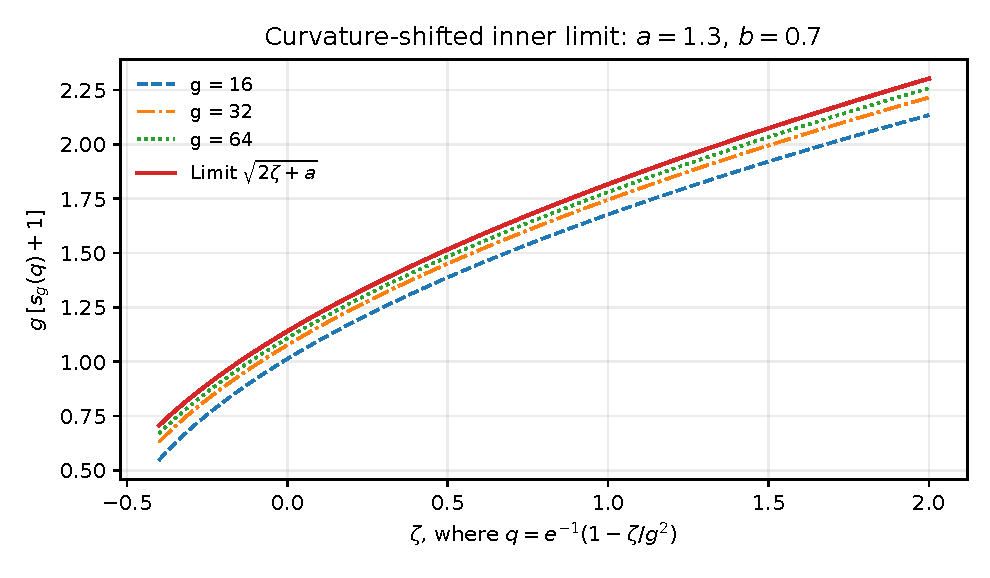
\includegraphics[width=.97\linewidth]{figures/fold_scaling.pdf}
\caption{The unshifted inner coordinate detects the logarithmic curvature. The ordinate is $g(s_g(q)+1)$ with $q=\e^{-1}(1-\zeta/g^2)$. The limiting curve is $\sqrt{2\zeta+a}$, not $\sqrt{2\zeta}$. The file \texttt{make\_figure.py} computes the exact roots and writes the $363$ plotted data points to CSV.}
\label{fig:inner}
\end{figure}

\Needspace{13\baselineskip}
\subsection{Reproduction and software boundaries}
From the extracted archive, run
\begin{verbatim}
python verify.py --out results
python make_figure.py
pdflatex -interaction=nonstopmode -halt-on-error article.tex
pdflatex -interaction=nonstopmode -halt-on-error article.tex
pdflatex -interaction=nonstopmode -halt-on-error article.tex
\end{verbatim}
The verification run used SymPy~1.14.0 and mpmath~1.3.0. A dependency list, a build script, the raw JSON report, and the figure data are included. No Lean source is supplied or claimed to have been compiled. No theorem relies on a floating-point equality test.

\section{A route toward formalization and certified implementation}
\label{sec:formalization}
The repository already distinguishes exact formalized interfaces from broader manuscript statements \cite{repo}. A realistic extension should preserve that discipline.

The finite transport calculation has three layers. First, the purely algebraic sector coefficients can be formalized in a truncated power-series ring. The identity \eqref{eq:jet-computation}, or a coefficient-level Lagrange theorem, would give exact finite jets. The existing Bell-coefficient interfaces are natural downstream consumers, but the present report does not assume that their APIs already contain the required theorem.

Second, the analytic branch certificate requires a complex disk, boundary separation, and a zero-counting or analytic implicit-function argument. The numerical bound \eqref{eq:numeric-certificate} is deliberately designed so that an implementation can certify elementary inequalities and a finite list of derivative bounds rather than sampling an unknown inverse. Remainder transport is then a separate interface from the formal coefficient calculation.

Third, Borel-plane continuation and summability need more than a formal series algebra. A future formalization of \cref{thm:core} would either import a suitably formalized summable implicit-function theorem or build its analytic estimates explicitly. It would be misleading to mark the resurgence conclusion formalized merely because the finite coefficient recurrence or the forward differential equation is checked.

A practical certificate object for a fixed evaluation point would contain the center $g$, a radius $\rho$, a proof that $F(g)=x$, a lower bound on $|F'(g)|$, an upper bound on $\sup|F''|$, perturbation boundary norms, a strict rational upper bound for $\chi$, and the desired truncation degree. The exact coefficients and the analytic tail estimate would then produce a proof-carrying inverse enclosure. A root known only approximately would require an additional residual-to-root enclosure before applying the centered formulas.

\section{Further research questions and proposed projects}
\label{sec:agenda}
The questions below are not all claimed to be open in the literature. They are concrete next problems for this analytic inversion program, with the boundary between proved and unproved parts stated explicitly.

\begin{problem}[Exact amplitude radius and complex singularities]
For the Euler--logarithm central map with real $a,b$, determine whether the nearest singularity of the selected amplitude inverse is always the real fold for all sufficiently large $g$. Prove or refute $R_g=q_{\mathrm c}(g)$. The present sandwich \eqref{eq:radiusbounds} proves only $R_g=\e^{-1}+O(g^{-2})$. A positive result, together with suitable continuation to a slit neighborhood, would support precise large-sector-order coefficient asymptotics.
\end{problem}

\begin{problem}[Local Borel singularities and bridge equations]
Determine the full singular germ of the Borel transform of $\widehat r$ at the first action and at its multiples, starting from the explicit kernel \eqref{eq:kernel}. Separate the pole contribution, logarithmic terms, and their nonlinear propagation. The exact finite Stokes jump fixes the lateral difference, but a complete local alien-calculus description needs additional analysis. At a resonant action, distinguish primitive from composite contributions rather than assuming a unique decomposition from the action label alone.
\end{problem}

\begin{problem}[Uniform optimal truncation through inversion]
Combine a least-term truncation bound for the Euler input with the inverse disk certificate to obtain a fully explicit, uniform hyperasymptotic error for $G_\pm$. The target should specify the truncation index, the angular dependence near the Stokes ray, and the interaction with the exponentially small sector truncation. Fixed algebraic order and fixed sector order are already controlled here; simultaneous large-order optimization is a separate problem.
\end{problem}

\begin{problem}[Gamma and Barnes-type exact cores]
Apply the exact-core kernel strategy to the Stirling correction in inverses of $\Gamma$ and Barnes-type functions. The challenge is not the formal residual recursion alone: one must choose the appropriate exponential--logarithmic core, identify the Borel singular lattice, and verify summable analytic-parameter bounds on a sector. Complex actions pointing in opposite directions make a naive positive-action semigroup argument inadequate.
\end{problem}

\begin{problem}[Coalescing actions and an action tending to zero]
The finite-action transport theorem is uniform under action coalescence as long as its norm certificate remains strict. Develop a double-scaling theory when $A\to0$ while $x\to\infty$. The effective parameter then involves $Ax$, and $\e^{-Ax}$ may no longer be flat on the original algebraic scale. Establish which renormalized core replaces the fixed-action construction and when sector ordering changes.
\end{problem}

\begin{problem}[Countably many resurgent input poles]
Find verifiable conditions on $(A_j,b_j)$ with $A_j\to\infty$ under which the countable analytic inverse of \cref{cor:countable} also has an exact-core resurgent correction. Normal convergence of the forward meromorphic Borel kernel and uniform parameter seminorm estimates are plausible starting hypotheses. They must be checked on lifted continuation paths, not just on the positive real axis.
\end{problem}

\begin{problem}[Pre-existing critical points of the forward map]
The amplitude fold in \cref{thm:radius} starts from $F'(g)>0$. Analyze inverse Stokes transport when the unperturbed forward map itself approaches a zero of $F'$. In that regime the linear certificate degenerates and exponentially small perturbations can become square-root or higher Puiseux effects. Construct a uniform multi-parameter model that separates a pre-existing forward critical point from the large-amplitude fold studied here.
\end{problem}

\begin{problem}[Certified recovery from approximate inverse data]
The recovery theorem uses exact partial inverses and an exact asymptotic limit. Design a finite-data algorithm with rigorous error bars when the inverse branches are known only numerically. The exponentially magnified normalization in \eqref{eq:recovery} creates a conditioning problem. Quantify required precision, the subtraction error from already recovered actions, and the loss of identifiability when two actions are close rather than exactly equal.
\end{problem}

\begin{problem}[Several dependent variables]
Replace the scalar forward map by a holomorphic map on $\C^m$ with an invertible Jacobian. Develop an analogue of the boundary-norm certificate and a rooted-tree formula for finite Stokes transport. Scalar commutativity of the additive transformations survives at the level of coherently inverted forward maps, but the explicit characteristic description and the geometry of critical Jacobian sets become substantially more complicated.
\end{problem}

\begin{problem}[Formalized analytic transport certificate]
Formalize a finite-degree version of \cref{thm:transport} with its tail bound, then the explicit Euler disk estimate. A useful milestone would be a Lean-checked enclosure for a nonreal lateral inverse with a certified real-averaging defect. This would connect the repository's exact-core and remainder interfaces to genuinely beyond-all-orders analytic data without claiming a full formalization of resurgence prematurely.
\end{problem}

\Needspace{12\baselineskip}
\section{Conclusion}
Formal inversion, analytic summation, and finite Stokes transport are distinct tasks. In the Euler--logarithm family they can be connected without conflating them. The exact logarithmic core turns the inverse correction into an ordinary resurgent implicit problem. The contour transport formula then determines every nonlinear sector from finite forward data and supplies a convergent analytic remainder bound. The same construction explains why naive averaging of lateral inverses introduces a positive exponentially small bias and why action resonances do not create new inverse constants.

The large-amplitude analysis identifies a second useful structure. A Lambert fold controls the asymptotic sector radius, but the logarithmic curvature shifts its inner scaling by $a/A$. The distinction between an outer $O(g^{-2})$ perturbation and its leading inner effect is quantified, not merely suggested by a formal expansion.

These are complete results for the hypotheses stated in this article. They are not a proof that arbitrary transseries are summable, a computation of every alien invariant of the repository's special functions, or a determination of the exact complex amplitude radius in all cases. The proposed next projects identify those remaining boundaries explicitly.

\appendix
\section{Notation and dependency guide}
\small
\begin{longtable}{@{}p{.22\linewidth}p{.73\linewidth}@{}}
\toprule
Symbol & Meaning\\
\midrule
\endhead
$F,G$ & A forward analytic map and its selected local inverse.\\
$G_{\bs}$ & Inverse of $F+\sum_j\sigma_j\phi_j$, with the branch fixed by the disk certificate.\\
$g,x$ & A base point and its image $x=F(g)$.\\
$\rho,m,\chi$ & Disk radius, forward boundary separation, and relative perturbation boundary norm.\\
$\bn,N,\bn!$ & A nonnegative multi-index, its total degree, and the product of its factorials.\\
$A_j,S_{\bn}$ & Primitive exponential actions and their nonnegative additive combination.\\
$U_{A,\pm}$ & Upper and lower Borel--Laplace sums of the positive-sign Euler series.\\
$F_\pm,G_\pm$ & Lateral forward maps and their inverses.\\
$\cF,\cG$ & Arithmetic average of the forward maps and its inverse; not an arbitrary median-summation convention.\\
$y=H_a(x)$ & Exact logarithmic core satisfying $y+a\log y=x$.\\
$\widehat r,r_\pm$ & Ordinary formal inverse correction in $y^{-1}$ and its lateral sums.\\
$\Omega$ & The locally finite additive semigroup generated by the positive input actions, including $0$.\\
$s,q,\psi_g$ & Normalized displacement, normalized amplitude, and normalized forward increment.\\
$\kappa_g,\eta_g$ & Dimensionless second and third forward derivatives.\\
$s_{\mathrm c},q_{\mathrm c},R_g$ & Real fold location, critical amplitude, and Taylor radius of the selected amplitude branch.\\
\bottomrule
\end{longtable}
\normalsize

\noindent\textbf{Logical dependencies.} The analytic inverse-transport theorem uses only standard one-variable complex analysis and is independent of the resurgent closure theorem. The exact-core resurgence theorem invokes the specified general implicit theorems after verifying their hypotheses. The finite inverse Stokes formula combines the transport theorem with the elementary Euler residue computation. The averaging and recovery results use the transport theorem and asymptotics. The fold results are local analytic consequences of the normalized derivative hypotheses and do not depend on Borel summability.

\Needspace{14\baselineskip}
\section{An exact residual interpretation of the real bias}
There is a second way to see the sign and order in \eqref{eq:averaging-defect}. Let $G_p=g+u(p)$, where the coefficients of $u$ are real and $p=\pi\ii b$. The linear correction $u_1p$ is imaginary. The quadratic correction is real and equals
\[
 p^2C_2=\pi^2b^2\e^{-2g}
 \left(\frac1{F'(g)^2}+\frac{F''(g)}{2F'(g)^3}\right).
\]
Here $G'=1/F'$ and $G''=-F''/(F')^3$ have been substituted. Both nonlinear mechanisms are visible: evaluating $\e^{-z}$ at the displaced root produces the term $1/F'^2$, while the curvature of the forward map produces $F''/(2F'^3)$. The first dominates at infinity. This also provides an implementation formula using only two forward derivatives.

For a general positive action $A$, replace the first term in parentheses by $A/F'^2$ and the exponential by $\e^{-2Ag}$. This decomposition shows why a purely first-order error-transport estimate cannot determine the real bias: its first-order imaginary correction averages to zero.

\begin{thebibliography}{9}
\raggedright
\bibitem{repo}
Vladimir Reshetnikov, \emph{ProveIt: Transseries---the polynomial--logarithmic calculus and its inversions}, repository inventory and formalization crosswalk, snapshot
\texttt{04e06e032dff1966513bfba316966d52db3646b4}, accessed 29 September 2026.
\url{https://github.com/VladimirReshetnikov/ProveIt/blob/04e06e032dff1966513bfba316966d52db3646b4/Analysis/FabiusFunction/docs/semi-formalized-research-frontiers/drafts/series-and-transseries/Transseries_And_Inversion/README.md}.

\bibitem{sauzin2015}
David Sauzin, \emph{Nonlinear analysis with resurgent functions}, Annales scientifiques de l'\'Ecole Normale Sup\'erieure (4) \textbf{48} (2015), no.~3, 667--702. In particular Theorems~4 and~$4'$ and Section~3.5.
\url{https://doi.org/10.24033/asens.2255}.
Author manuscript: \url{https://arxiv.org/abs/1212.4477}.

\bibitem{sauzin2014}
David Sauzin, \emph{Introduction to 1-summability and resurgence}, arXiv:1405.0356, 2014.
\url{https://arxiv.org/abs/1405.0356}.

\bibitem{edgar}
Gerald A. Edgar, \emph{Transseries: Composition, Recursion, and Convergence}, arXiv:0909.1259, 2009.
\url{https://arxiv.org/abs/0909.1259}.

\bibitem{dlmf}
NIST Digital Library of Mathematical Functions, \emph{Section 4.13: Lambert $W$-Function}, consulted 29 September 2026.
\url{https://dlmf.nist.gov/4.13}.
\end{thebibliography}
\end{document}
